\documentclass[12pt]{article}
\usepackage{tikz}
\usepackage{caption} % Include the caption package
\usepackage{tcolorbox} % For creating boxed environments
\tcbuselibrary{skins, breakable} % Allows boxes to break across pages and use skins

\usepackage[margin=1in]{geometry} % Adjust the overall text width

\begin{document}

\setcounter{figure}{1} % Set the counter to 1 so that the next figure is Figure 2

\begin{tcolorbox}[colback=gray!5!white, colframe=black!75!black, boxrule=1pt, breakable,
                  left=5pt, right=5pt, top=10pt, bottom=10pt, width=0.5\textwidth, 
                  enlarge right by=1.5mm, title=Figure 2. Example of a 2 x 2 x 2 Tensor of Real Numbers]
\centering
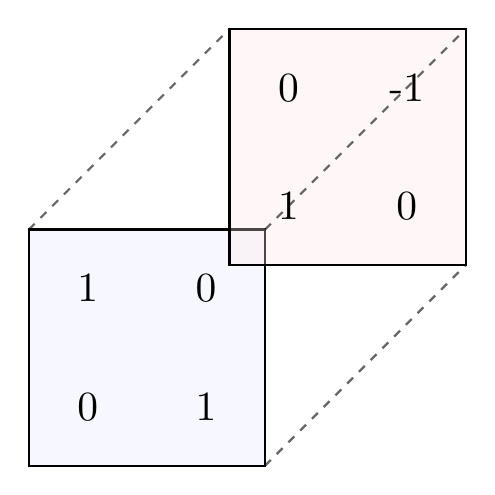
\begin{tikzpicture}[scale=1.5, every node/.style={scale=1.5}]
    % Lower matrix
    \draw[thick, fill=blue!10!white, fill opacity=0.3] (0,0) rectangle (2,2);
    \node at (0.5, 1.5) {1};
    \node at (1.5, 1.5) {0};
    \node at (0.5, 0.5) {0};
    \node at (1.5, 0.5) {1};

    % Upper matrix
    \begin{scope}[shift={(1.7,1.7)}]
        \draw[thick, fill=red!10!white, fill opacity=0.3] (0,0) rectangle (2,2);
        \node at (0.5, 1.5) {0};
        \node at (1.5, 1.5) {-1};
        \node at (0.5, 0.5) {1};
        \node at (1.5, 0.5) {0};
    \end{scope}

    % Dashed lines with opacity for a cleaner look
    \draw[dashed, thick, opacity=0.6] (2,0) -- (3.7,1.7);  % From bottom right corner of lower to bottom right corner of upper
    \draw[dashed, thick, opacity=0.6] (2,2) -- (3.7,3.7);  % From top right corner of lower to top right corner of upper
    \draw[dashed, thick, opacity=0.6] (0,2) -- (1.7,3.7);  % From top left corner of lower to top left corner of upper
\end{tikzpicture}

\bigskip % Add some space before the caption

\refstepcounter{figure} % Increase figure counter
\begin{minipage}[t]{\linewidth} % Set the caption width to the box width
    \textbf{Figure \thefigure.} This figure is an example of a 2 x 2 x 2 tensor of real numbers. The two frontal matrix slices are colored distinctly. There are relationships between the frontal slices and the horizontal slices (not colored) as well as relationships between the two-dimensional slices and the rows, columns, and pillars. Tensors should be treated as a single entity to preserve information encoded in these fundamental relationships.
\end{minipage}
\end{tcolorbox}

\end{document}
